\documentclass[a4paper]{scrreprt}
\usepackage[T1]{fontenc}
\usepackage[utf8]{inputenc}
\usepackage[ngerman]{babel}
\usepackage{natbib}
%\usepackage{biblist}
\usepackage[procnames]{listings}
\usepackage{xcolor}
\usepackage{graphicx}


\definecolor{keywords}{RGB}{255,0,90}
\definecolor{comments}{RGB}{0,0,113}
\definecolor{red}{RGB}{160,0,0}
\definecolor{green}{RGB}{0,150,0}
 
%\lstset{language=Python, 
%        basicstyle=\ttfamily\small, 
%        keywordstyle=\color{keywords},
%        commentstyle=\color{comments},
%        stringstyle=\color{red},
%        showstringspaces=false,
%        identifierstyle=\color{green},
%        procnamekeys={def,class}}
\lstset{
  language=Python,
  tabsize=4,
  captionpos=b,
  numbers=left,
  commentstyle=\color{green},
  backgroundcolor=\color{white},
  numberstyle=\color{gray},
  keywordstyle=\color{blue} \textbf,%otherkeywords={xdata},
  keywords=[2]{xdata},
  keywordstyle=[2]\color{red}\textbf,
  identifierstyle=\color{black},
  stringstyle=\color{red}\ttfamily,
  basicstyle = \ttfamily \color{black} \footnotesize,
  inputencoding=utf8/latin1,
  showstringspaces=false ,
  moredelim=[is][\color{yellow}]{|}{|},
}

\begin{document}


\author{Balk, Bastian; Herr David; Klause, Fabian; Frau Qian}
\title{Auswirkung von Elektrogeräten auf Power Line Communications} 
\maketitle

%%%%%%%%%%%%%%%Zitate
\nocite{Zitat01}
\nocite{Zitat02}
\nocite{PLC}






\begin{abstract}
\noindent Ziel dieser Arbeit ist eine Übersicht verschiedener PLC-Module und deren Anfälligkeit auf verschiedene zielgerichtete Störungen.
Folgende Modems standen hierbei zur Verfügung.

\begin{enumerate}
\item HomePlug AV
\item HomePlug 1.0
\item UPA
\end{enumerate}
Mithilfe eines Versuchbrettes wurden folgende Szenarien untersucht.

\begin{figure}[!htp]
\centering
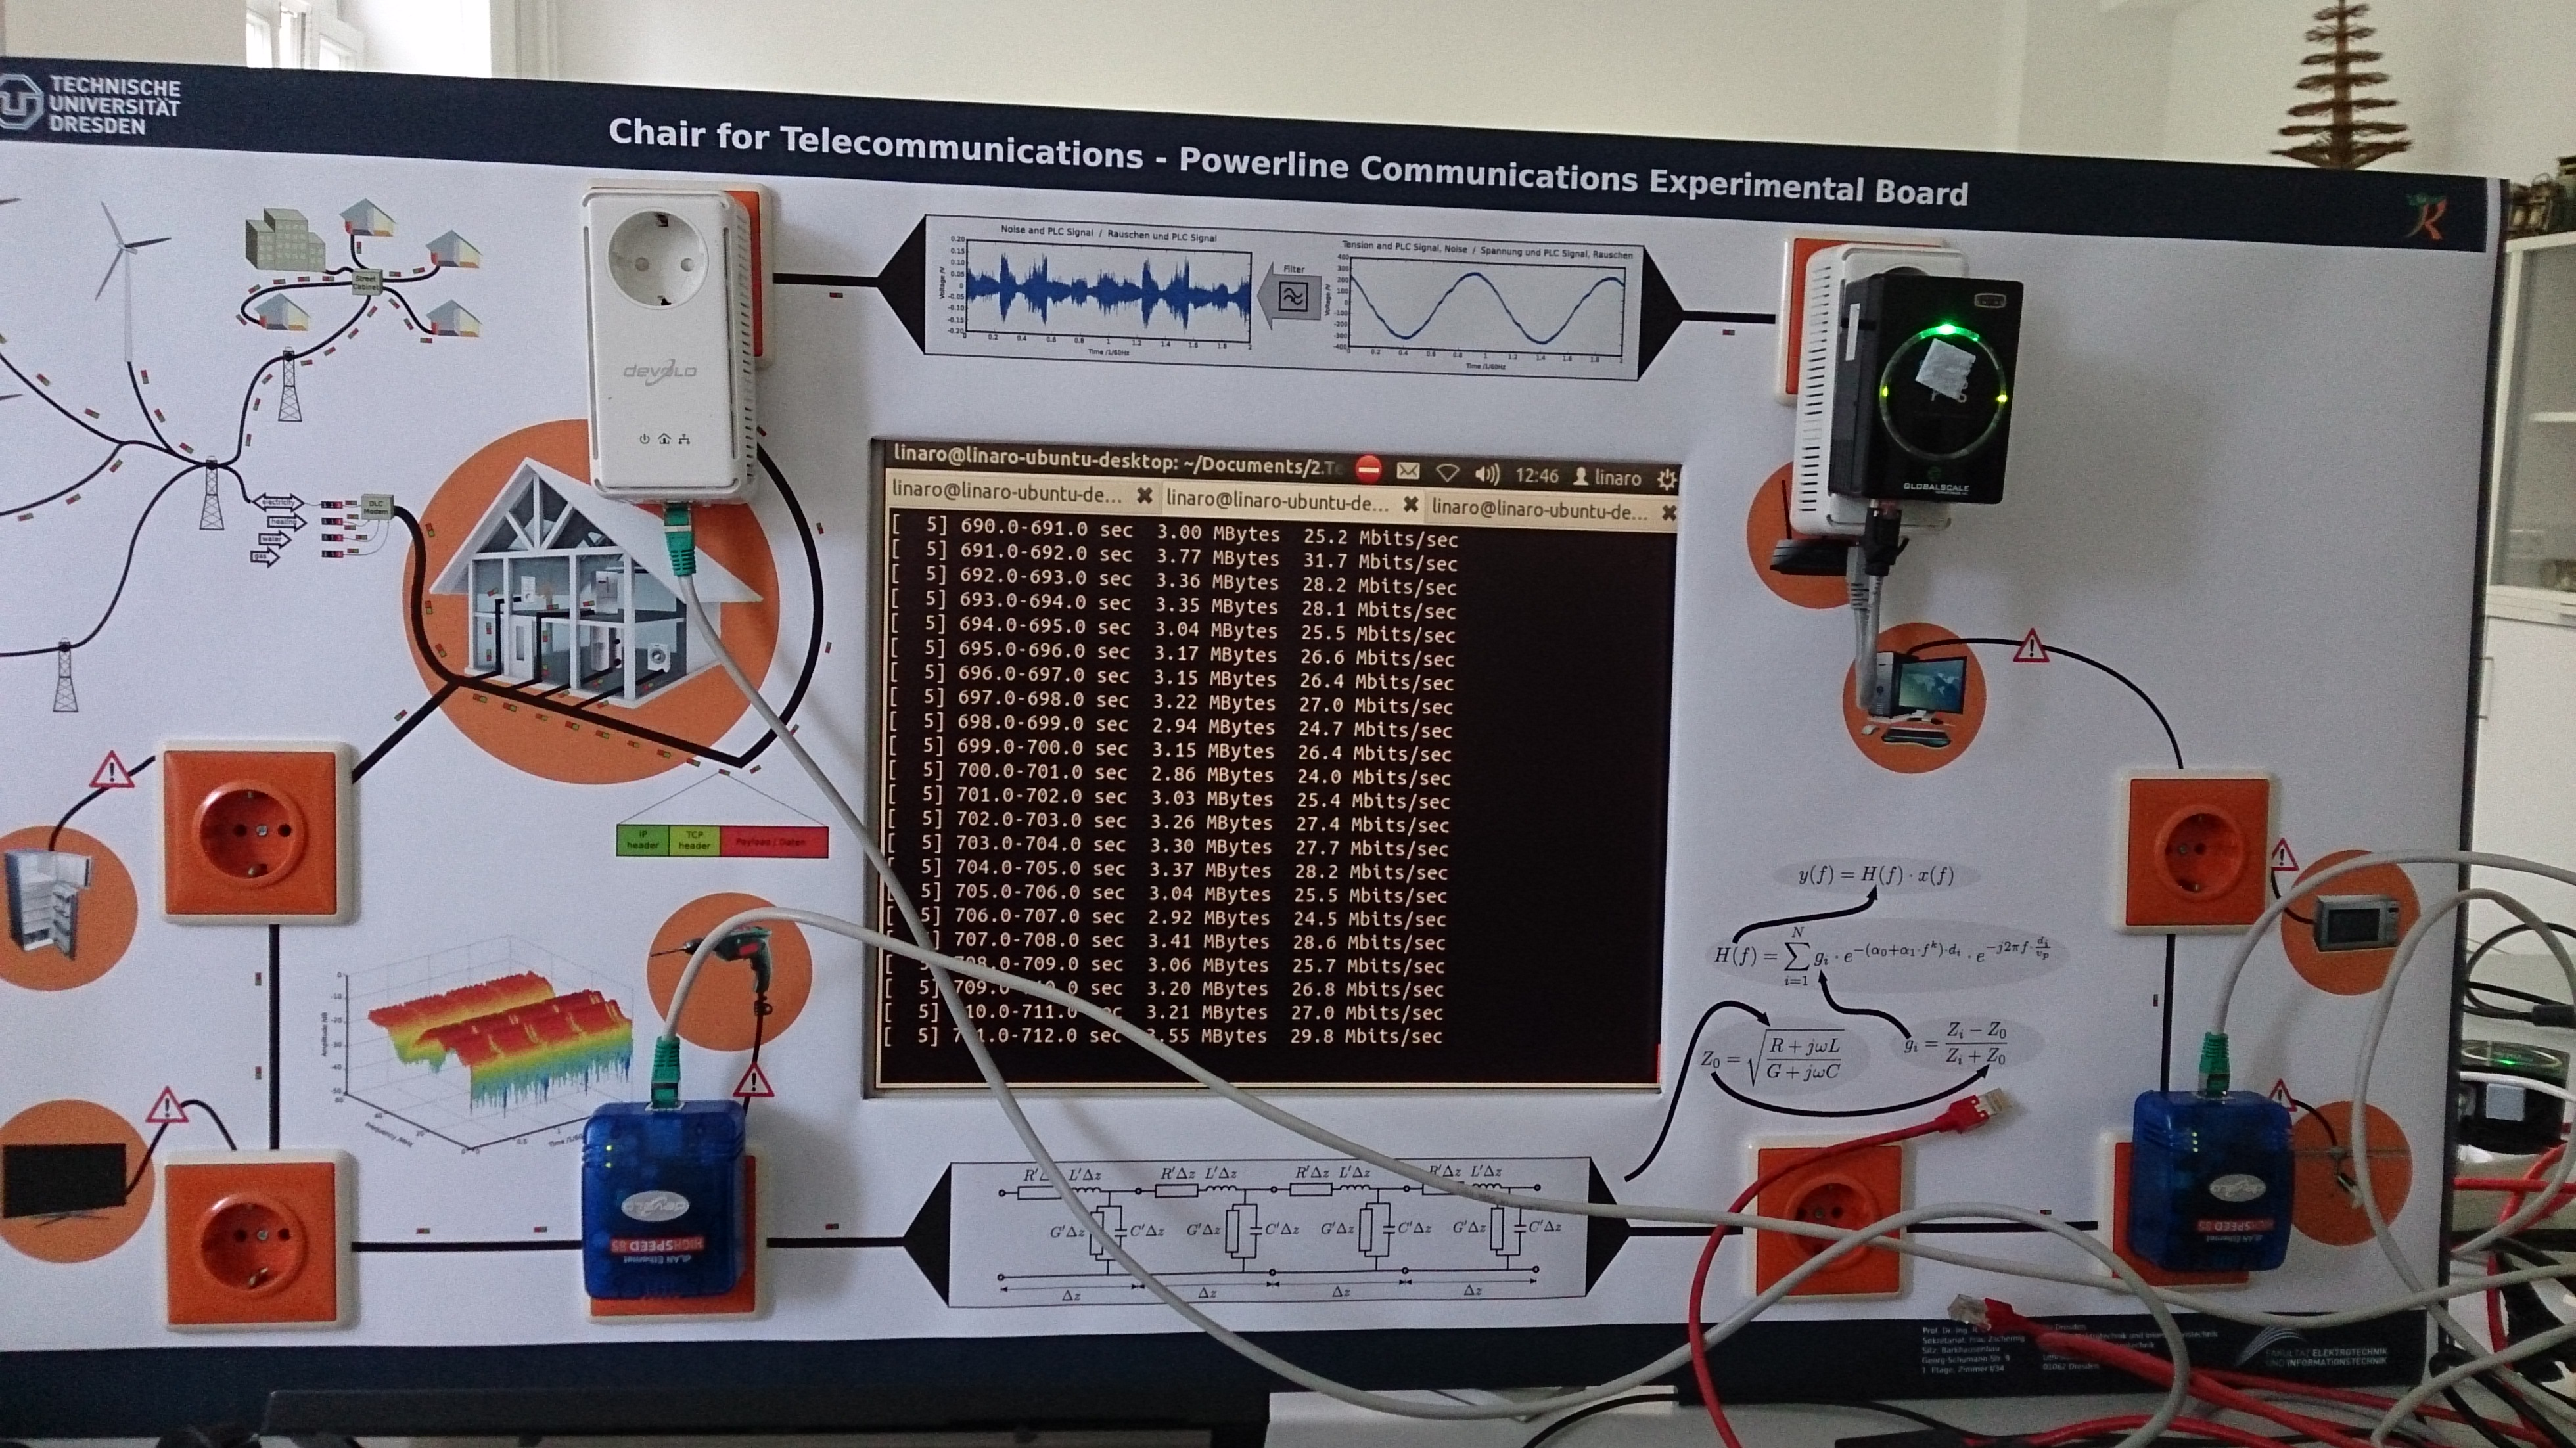
\includegraphics[scale=0.1]{./PLC.JPG}
\caption{Versuchsbrett}
\label{fig:PLC}
\end{figure}

\begin{enumerate}
\item Einfluss des externen Stromnetz 
\item Einfluß von elektrischen Geräten 
\item Koexistenz der zu untersuchenden PLC-Technologien
\item Einfluß von Distanz zwischen PLC Modems auf Netzwerkperformance
\end{enumerate}

Die Ergebnisse und deren Analyse werden im Folgenden genau behandelt.
\end{abstract} 


\tableofcontents 
\chapter{Grundlagen}
Die generelle Funktionsweiße von PLC basiert darauf, dass auf die Standard-Netzspannung von 50 Hz ein höherfrequentes analoges Signal überlagert wird.
Der CENELEC-Standard EN50065-1 weißt der PLC-Technik vier Bänder zwischen 3 kHz und 148,5 kHz zu. Wobei der Bereicht von 3 bis 95 khZ außerhalb der Wohnung vorgesehen ist. \cite{Zitat01}

Um die Daten zu Übertragen bieten sich verschiendene Modulationsmöglichkeiten an. Die OFDM-Methode spielt hierbei eine ganz entscheidene Rolle.

\section{OFDM, Orthogonal Frequency-Division Multiplexing}
Bei OFDM wird das verfügbare Spektrum in viele kleine Subkanäle unterteilt, siehe Formel \ref{eq:Formel}. Auf denen jeweils ein Teil des Datenstroms überragen wird.So kann entsptrechend der Störungen den einzelnen Kanälen mehr oder weniger Datenstrom zugeteilt werden. Demnach ist dieses Verfahren besonders Robust gegen Störungen.
Ein wichtiger Bestandteil dieses Verfahren ist die Orthogonalität,siehe Abbildung \ref{fig:OFDM}. Diese ist auch hauptveranwortlich für die sehr gute spektralle Effizienz.\cite{Zitat02}
 
\begin{quotation}
  "Hohe spektrale Effizienz ist für den Erfolg schneller Powerline-Kommunikation wegen der begrenzten spektralen Ressourcen unverzichtbar. \cite{Zitat02}"
\end{quotation}
%Der einzige Nachteil gegenüber FH(Frequency Hopping) ist die stark schwankende Signalamplitude (Zitat: seite 250)


\chapter{Auswertung}
\section{Skript}

%\lstinputlisting{./plotDEM.py}
\input{Auswertung}


\begin{figure}[!htp]
\centering
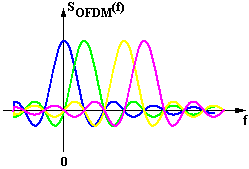
\includegraphics[scale=0.6]{./OFDM.png}
\caption{Orthogonal Frequency-Division Multiplexing}
\label{fig:OFDM}
\end{figure}

\begin{equation}
\label{eq:Formel}
 \Delta f = \frac{B}{N}

\end{equation}



\bibliographystyle{unsrt}
\bibliography{sources}

\end{document}
